\documentclass{article}
\usepackage{graphicx} % Required for inserting images
\usepackage{polski}
\usepackage{geometry}
\usepackage{graphicx}
\usepackage{float}

\geometry{
    a4paper,
    total={190mm,277mm},
    left=10mm,
    top=10mm,
}

\newenvironment{itemize.zip}
{ \begin{itemize}
    \setlength{\itemsep}{0pt}
    \setlength{\parskip}{0pt}
    \setlength{\parsep}{0pt}     }
{ \end{itemize}                  }

\title{\fontsize{20}{22}\selectfont Projekt zespołowy\\ część 1\\Strona internetowa z przepisami kulinarnymi\\"Wika gotuje"}
\date{}

\begin{document}

\section{Projekt interfejsu użytkownika}
\textit{Przedstawione poniżej zdjęcia interfejsów reprezentują tylko widoki na ekranie komputera, wersje mobilne zostały pominięte dla zredukowania rozmiaru tego dokumentu. Oczywiście
finalna wersja projektu będzie dopasowywać się do posiadanego rozmiaru posiadanego ekranu. \underline{Jako iż niektóre zdjęcią są bardzo duże jeśli chodzi o ich wysokość, załączono
również je osobno.}}

\subsection{Strona główna}
\begin{figure}[H]
    \begin{center}
        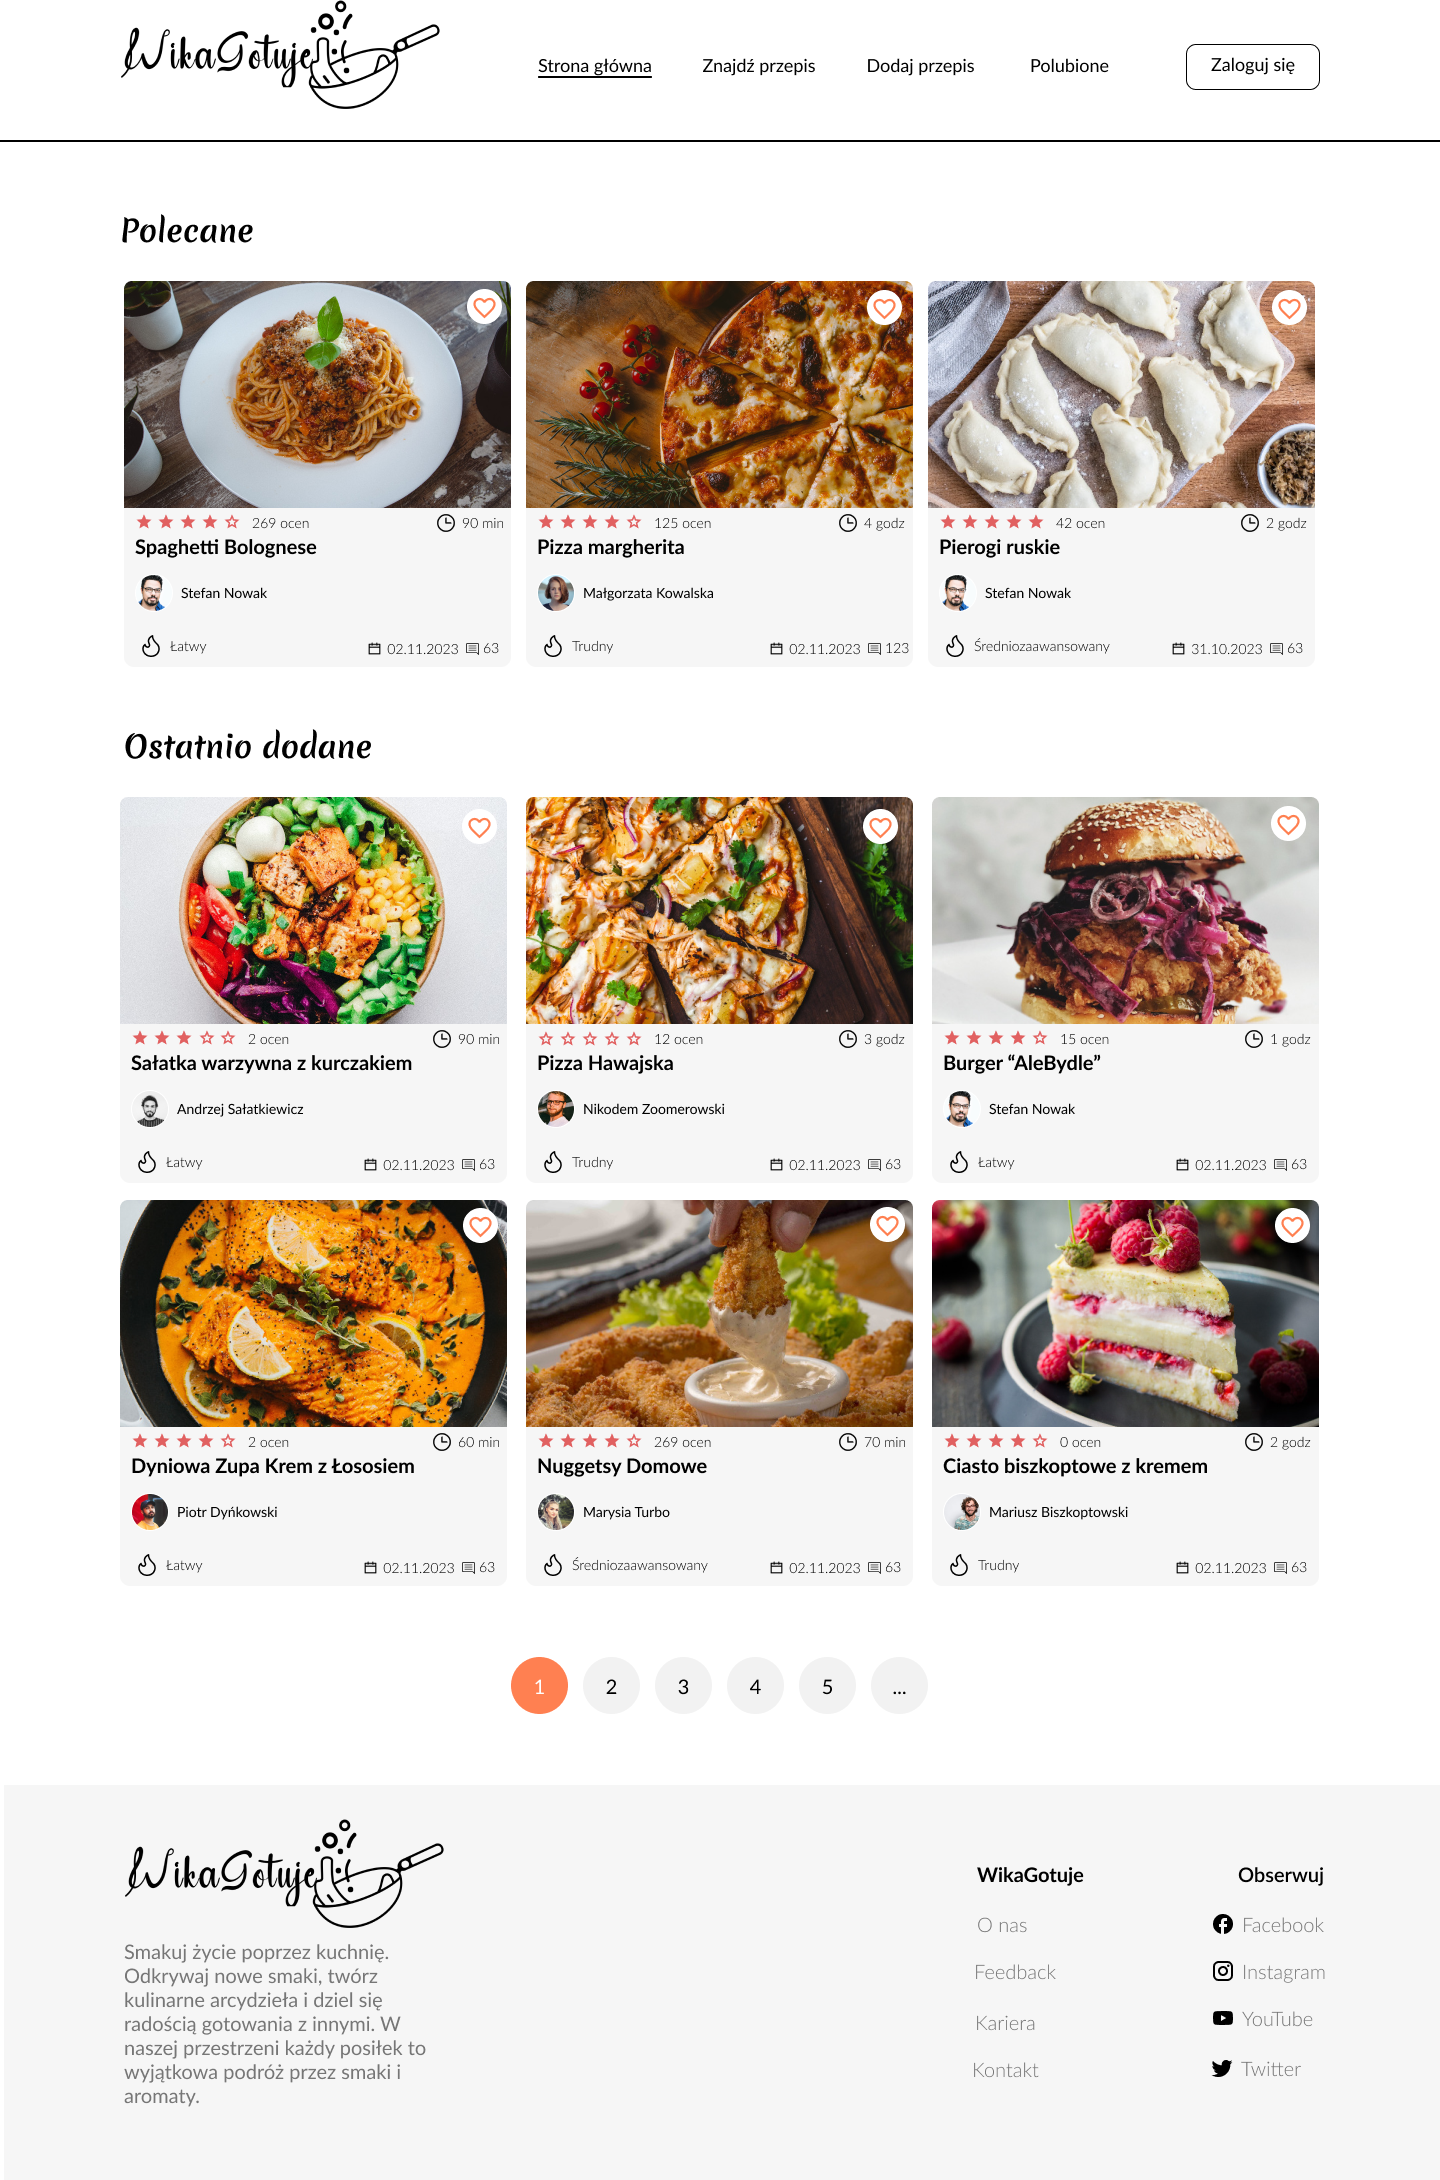
\includegraphics[width=0.79\textwidth]{mockups/main_page}
    \end{center}
    \caption{Widok strony głównej witryny; jest to pierwszy ekran jaki będzie dane zobaczyć potencjalnemu użytkownikowi}
    \label{fig:main_page}
\end{figure}
    
\newpage

\subsection{Strona podglądu danego przepisu}
\begin{figure}[H]
    \begin{center}
        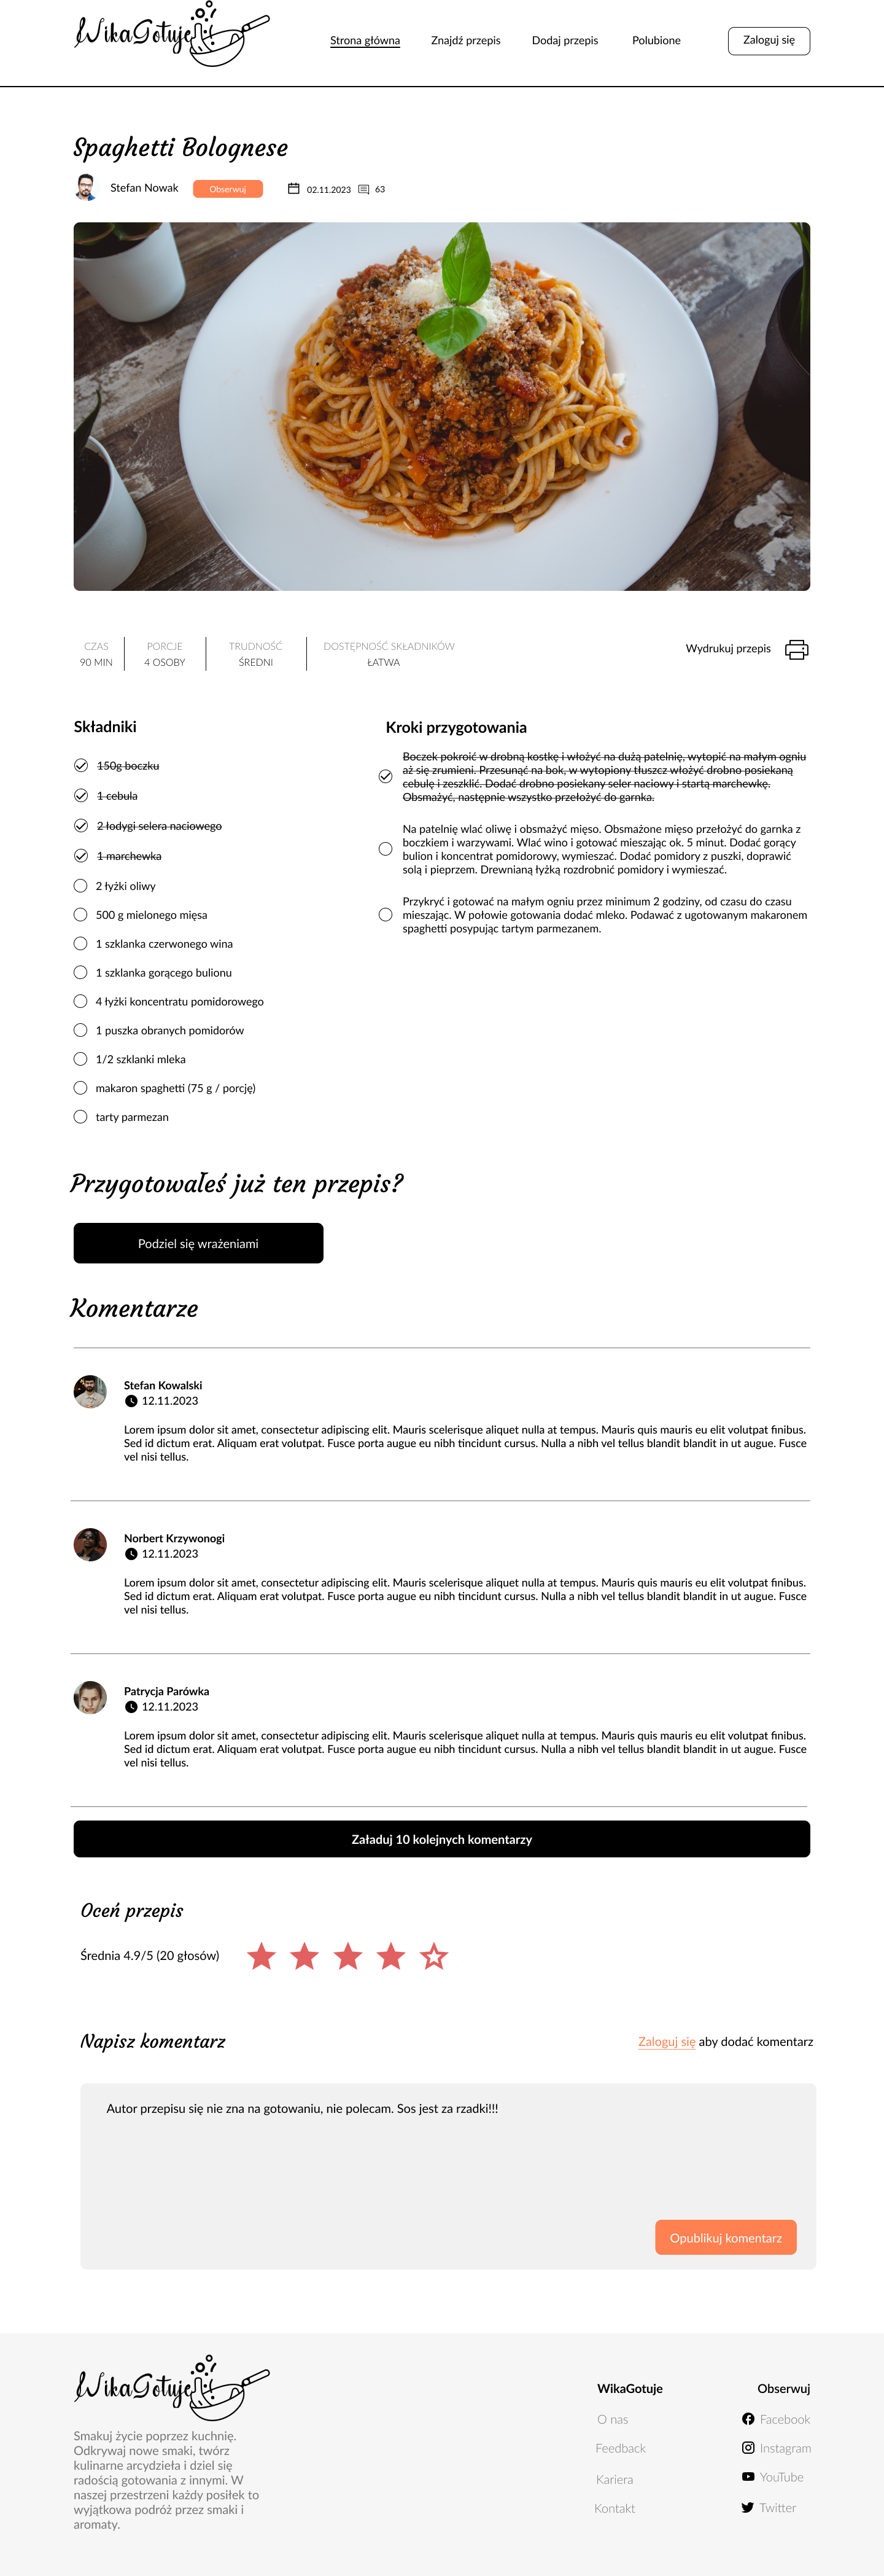
\includegraphics[width=0.45\textwidth]{mockups/recipe_preview}
    \end{center}
    \caption{Na tej stronie użytkownik może poznać dokładne informacje dotyczące przepisu, a także przejrzeć komentarze lub zostawić własną ocenę.}
\end{figure}

\newpage

\subsection{Strona dodawania nowego przepisu}

\begin{figure}[H]
    \begin{center}
        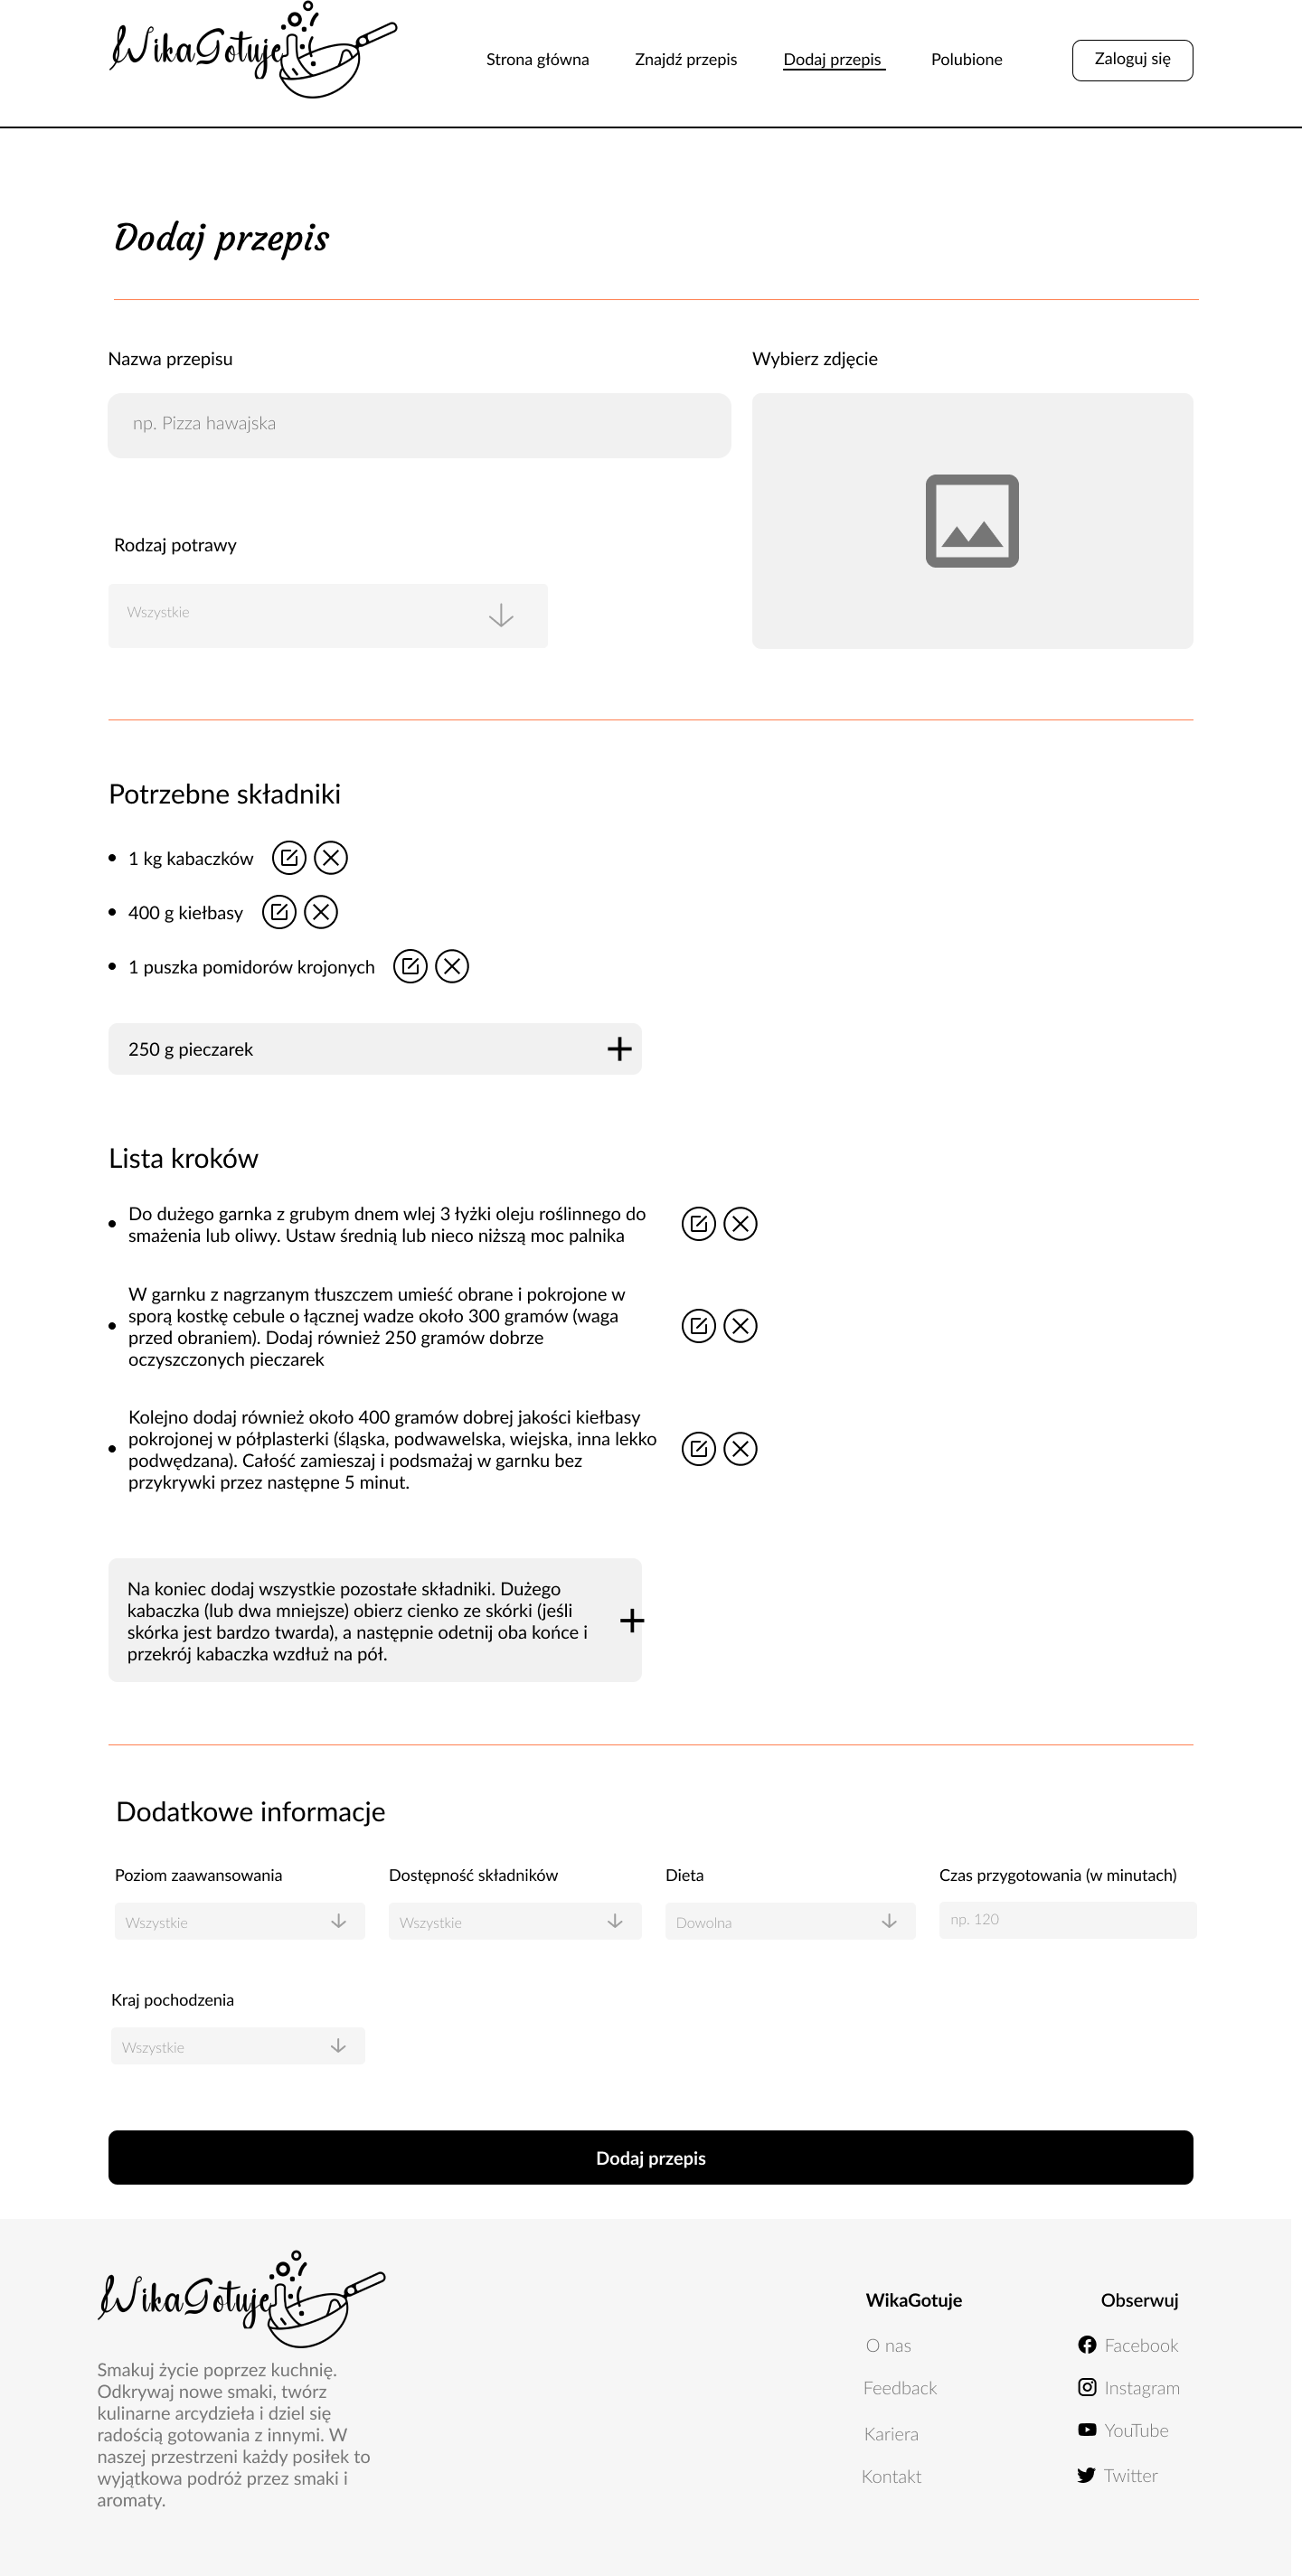
\includegraphics[width=0.65\textwidth]{mockups/adding_recipe}
    \end{center}
    \caption{Powyższa strona umożliwia użytkownikowi dodanie nowego przepisu, wraz ze zdjęciem gotowej potrawy, a także precyzyjnymi informacjami na jej temat}
    \label{fig:add_recipe}
\end{figure}

\newpage

\subsection{Strona służąca do znalezienia przepisu zgodnego z własnymi preferencjami}

\begin{figure}[H]
    \begin{center}
        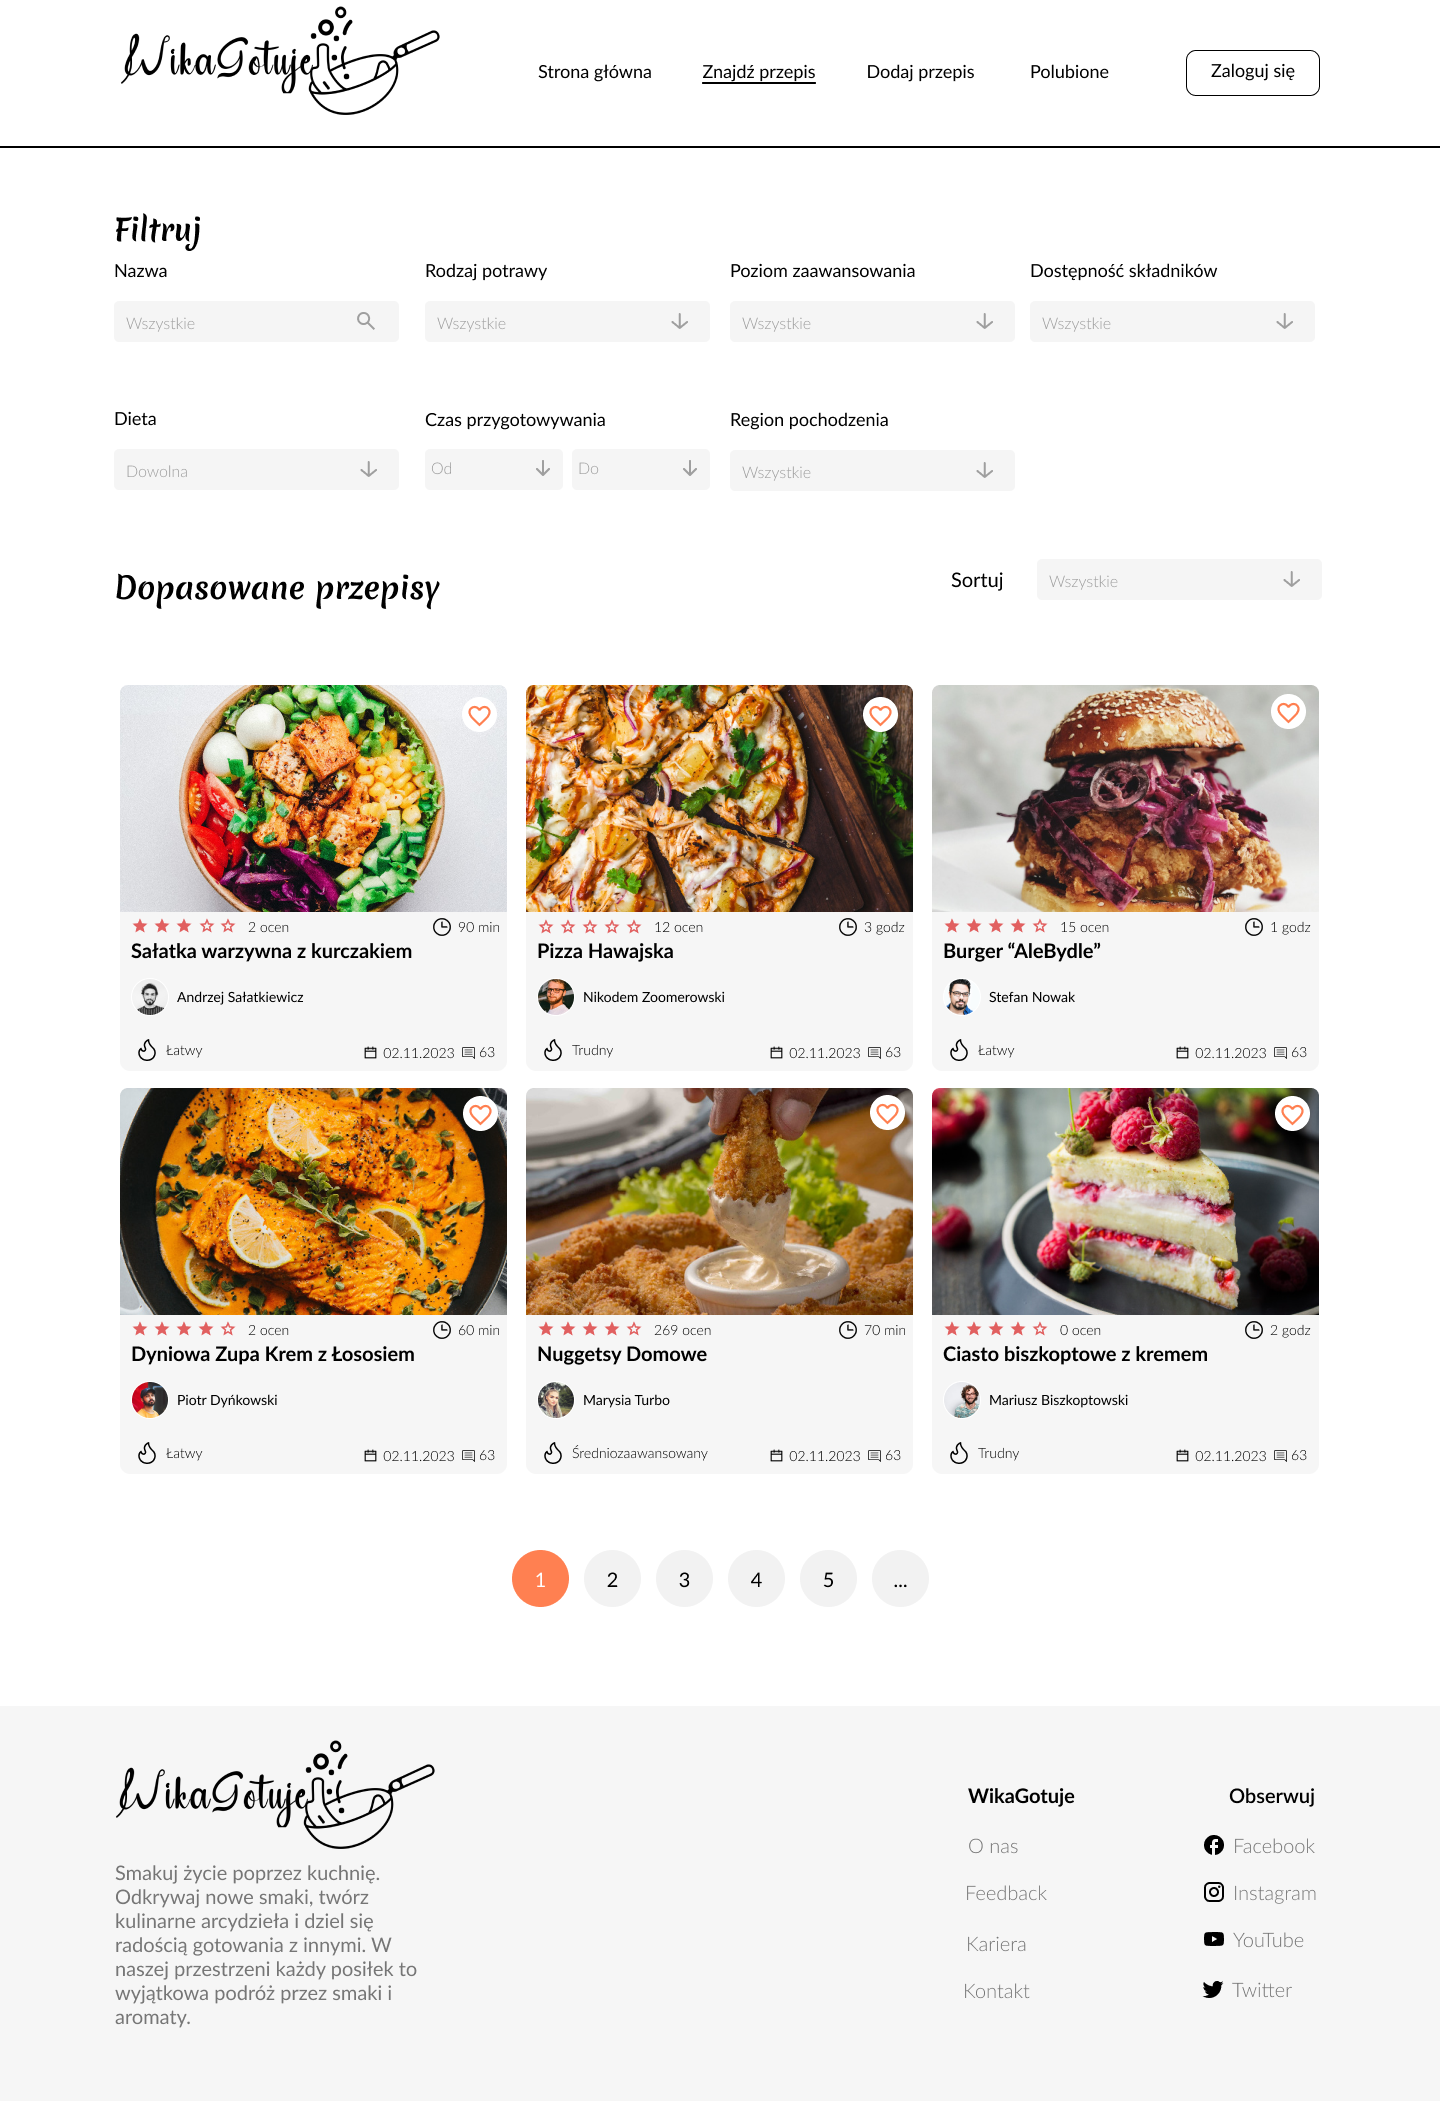
\includegraphics[width=0.9\textwidth]{mockups/find_recipe}
    \end{center}
    \caption{Widok podstrony umożliwiającej znalezienie przepisu zgodnego z nałożonymi filtrami.}
    \label{fig:find_recipe}
\end{figure}

\newpage

\subsection{Strona z zapisanymi przepisami lub tymi, które pochodzą od obserwowanych osób}

\begin{figure}[H]
    \begin{center}
        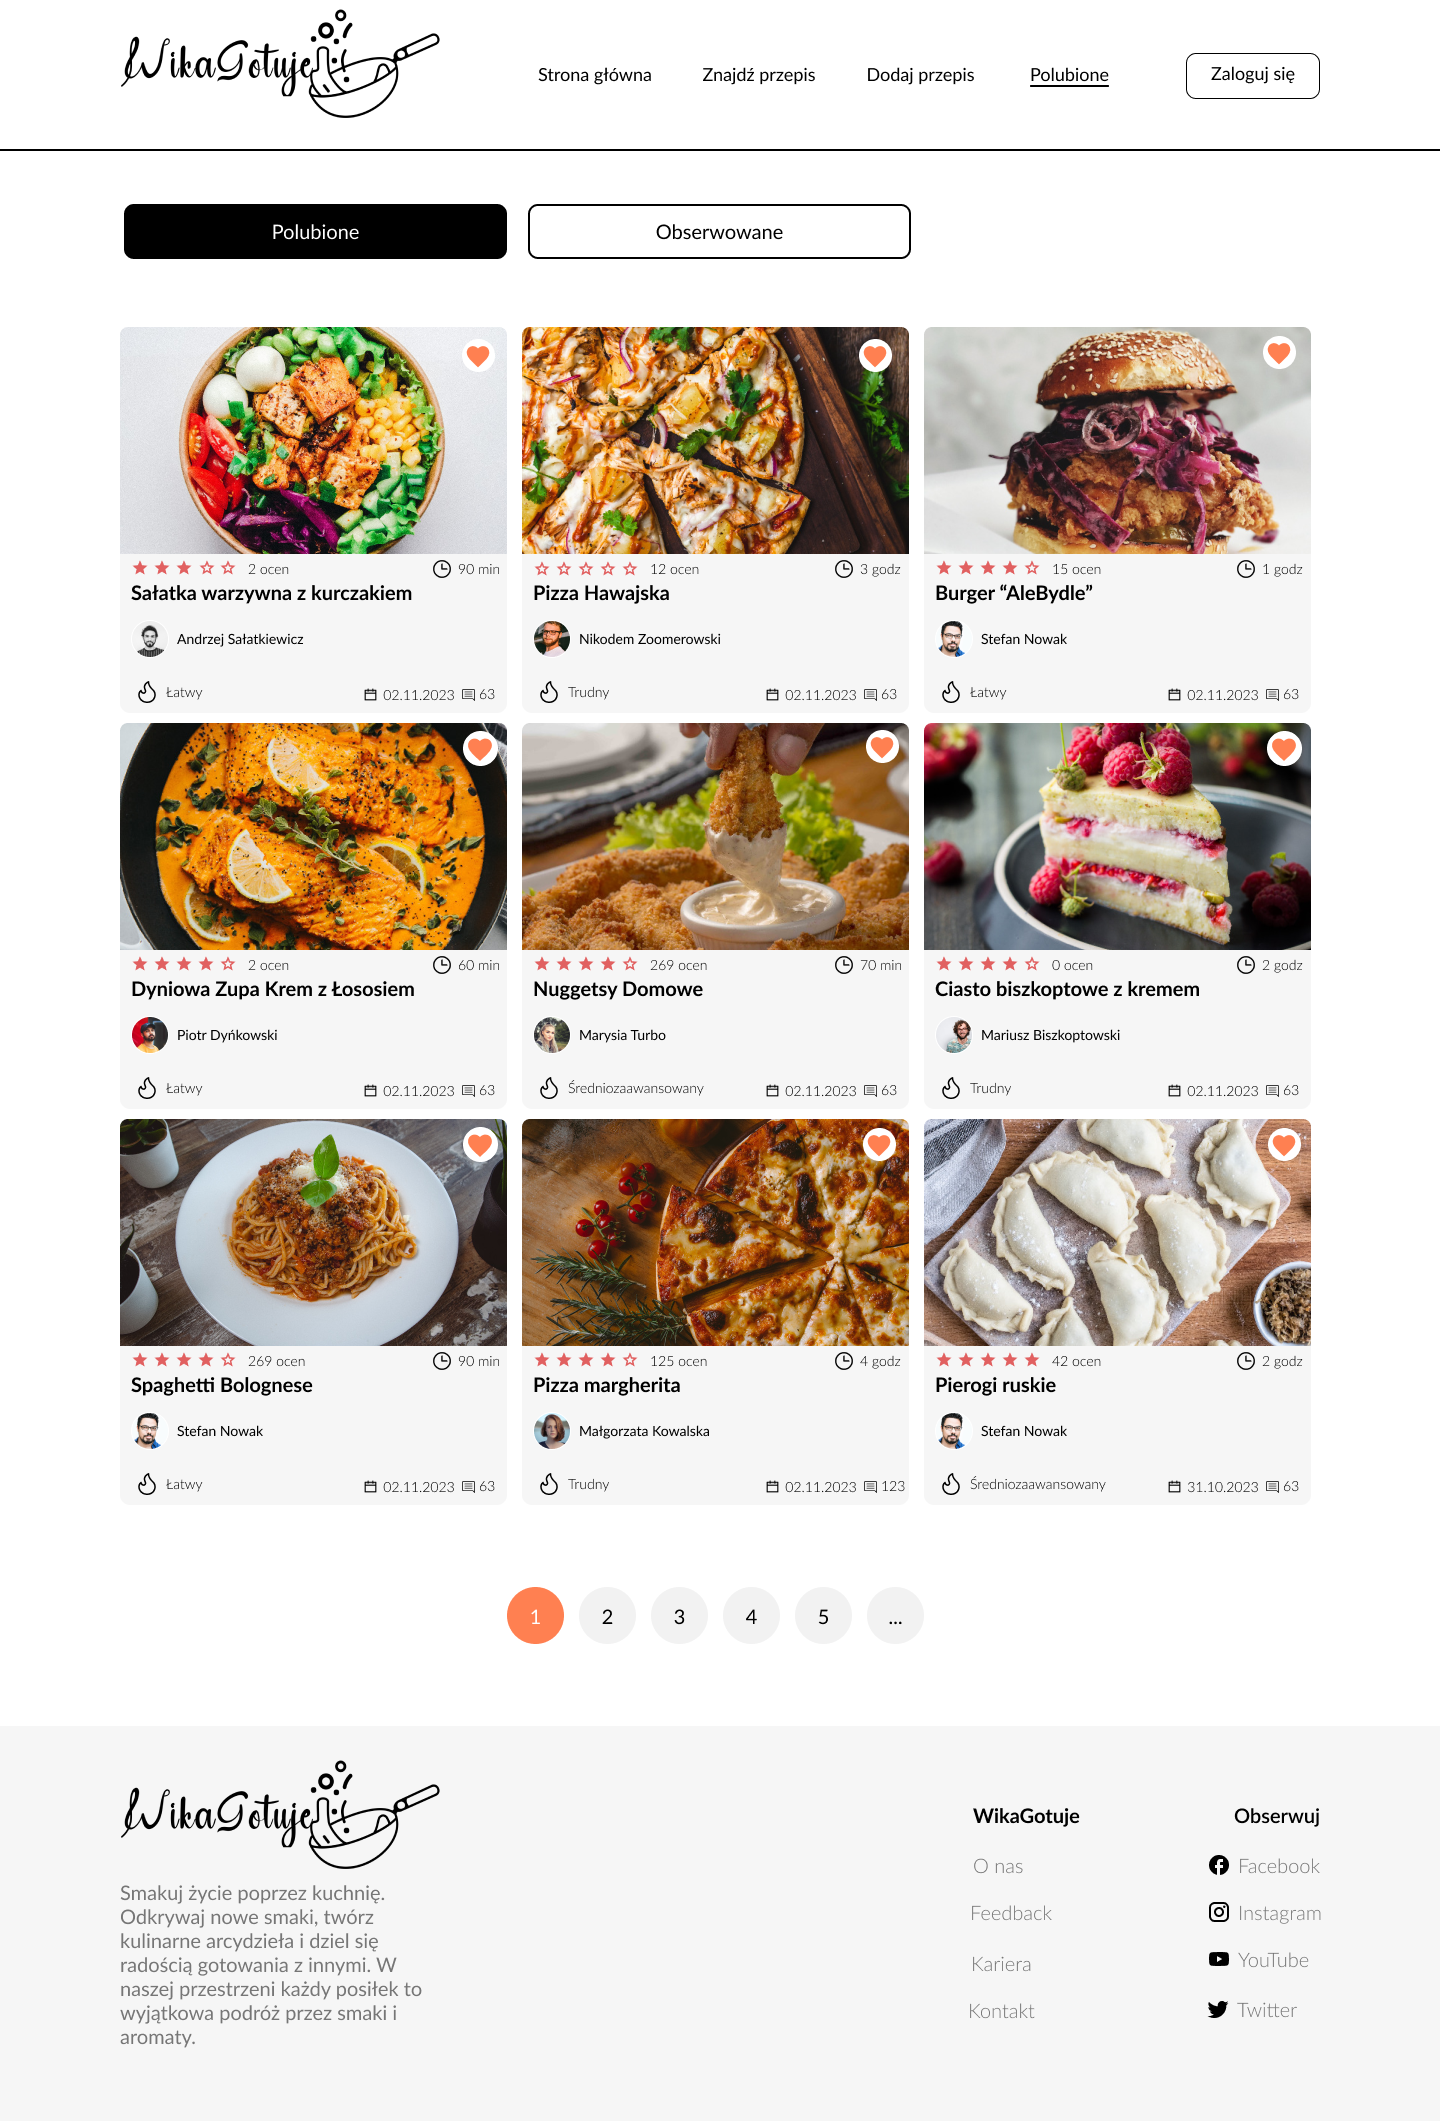
\includegraphics[width=0.9\textwidth]{mockups/saved_recipies}
    \end{center}
    \caption{Widok podstrony z zapisanymi/obserwowanymi przepisami}
\end{figure}

\newpage

\subsection{Strona własnego profilu}

\begin{figure}[H]
    \begin{center}
        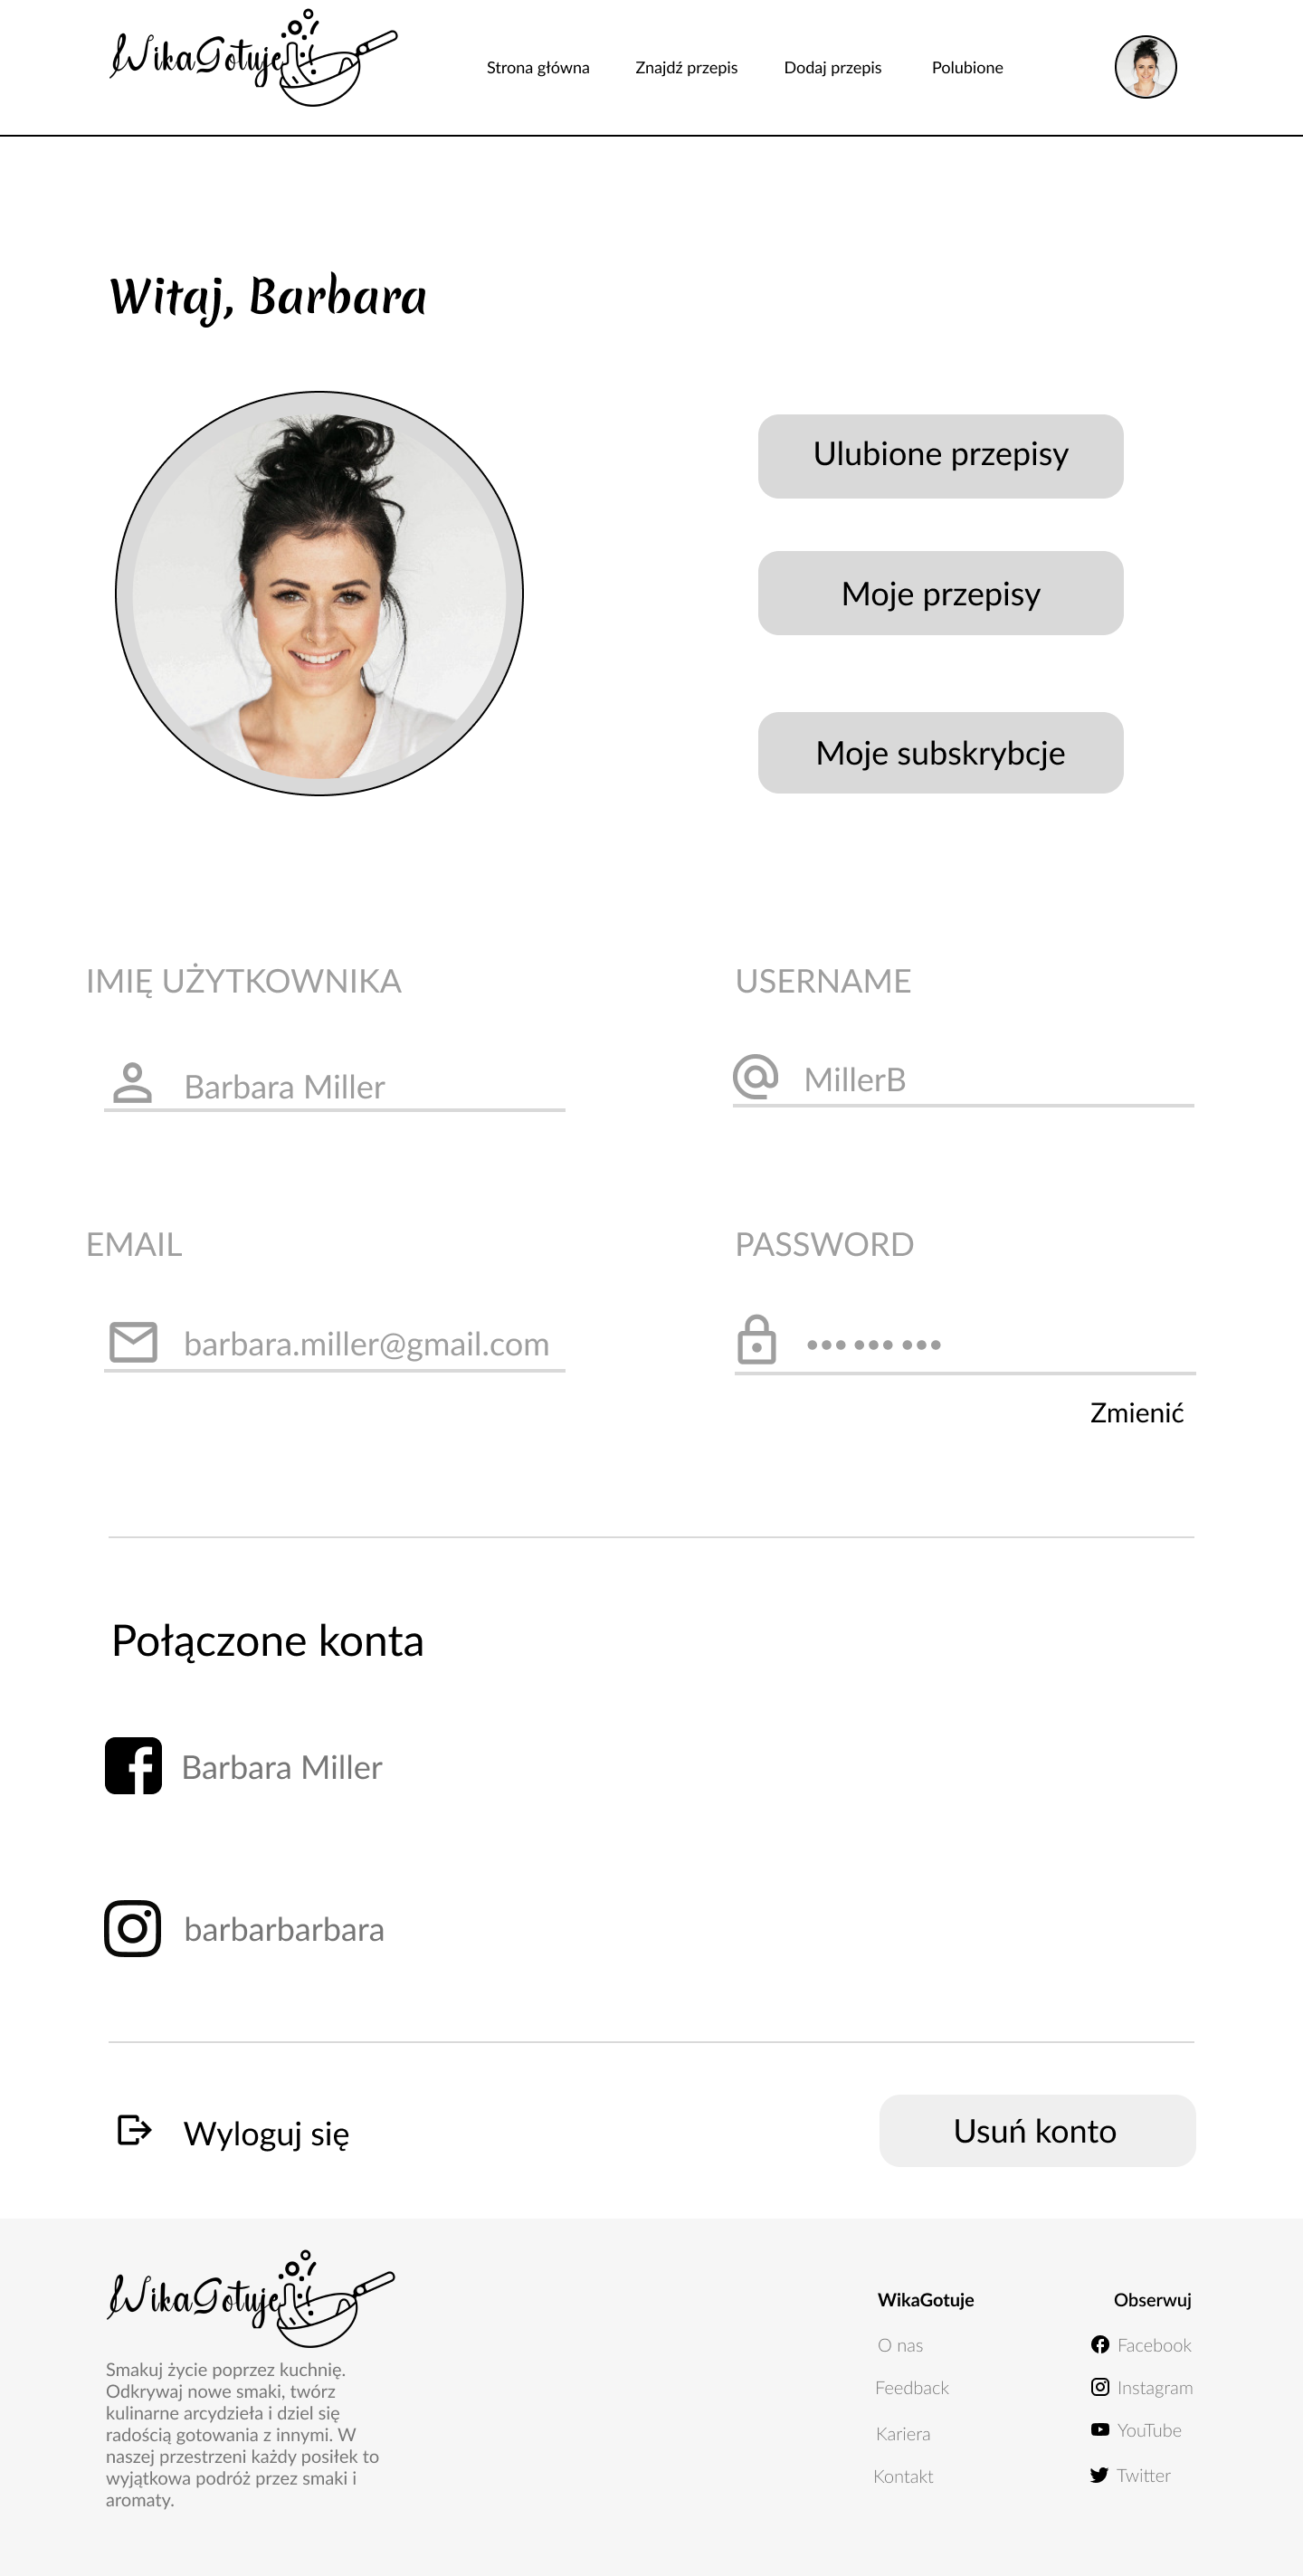
\includegraphics[width=0.65\textwidth]{mockups/user_profile}
    \end{center}
    \caption{Widok profilu użytkownika}
\end{figure}
\newpage

\subsection{Strona logowania}

\begin{figure}[H]
    \begin{center}
        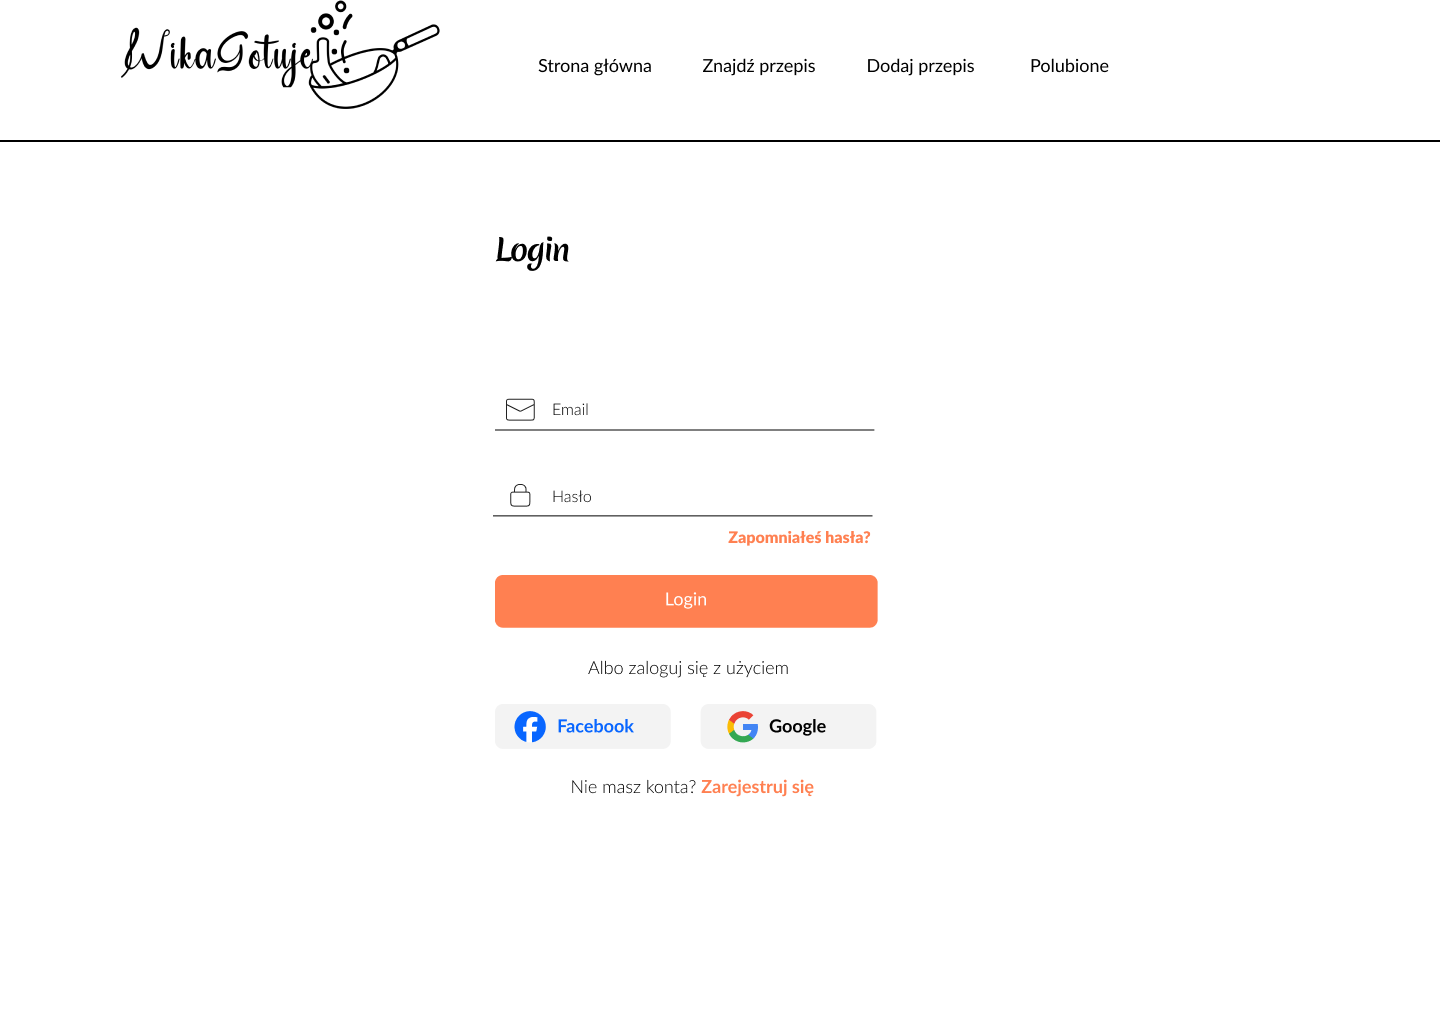
\includegraphics[width=0.8\textwidth]{mockups/login_page}
    \end{center}
    \caption{Widok podstrony odpowiedzialnej za logowanie użytkownika}
    \label{fig:login_page}
\end{figure}

\subsection{Strona rejestrowania}

\begin{figure}[H]
    \begin{center}
        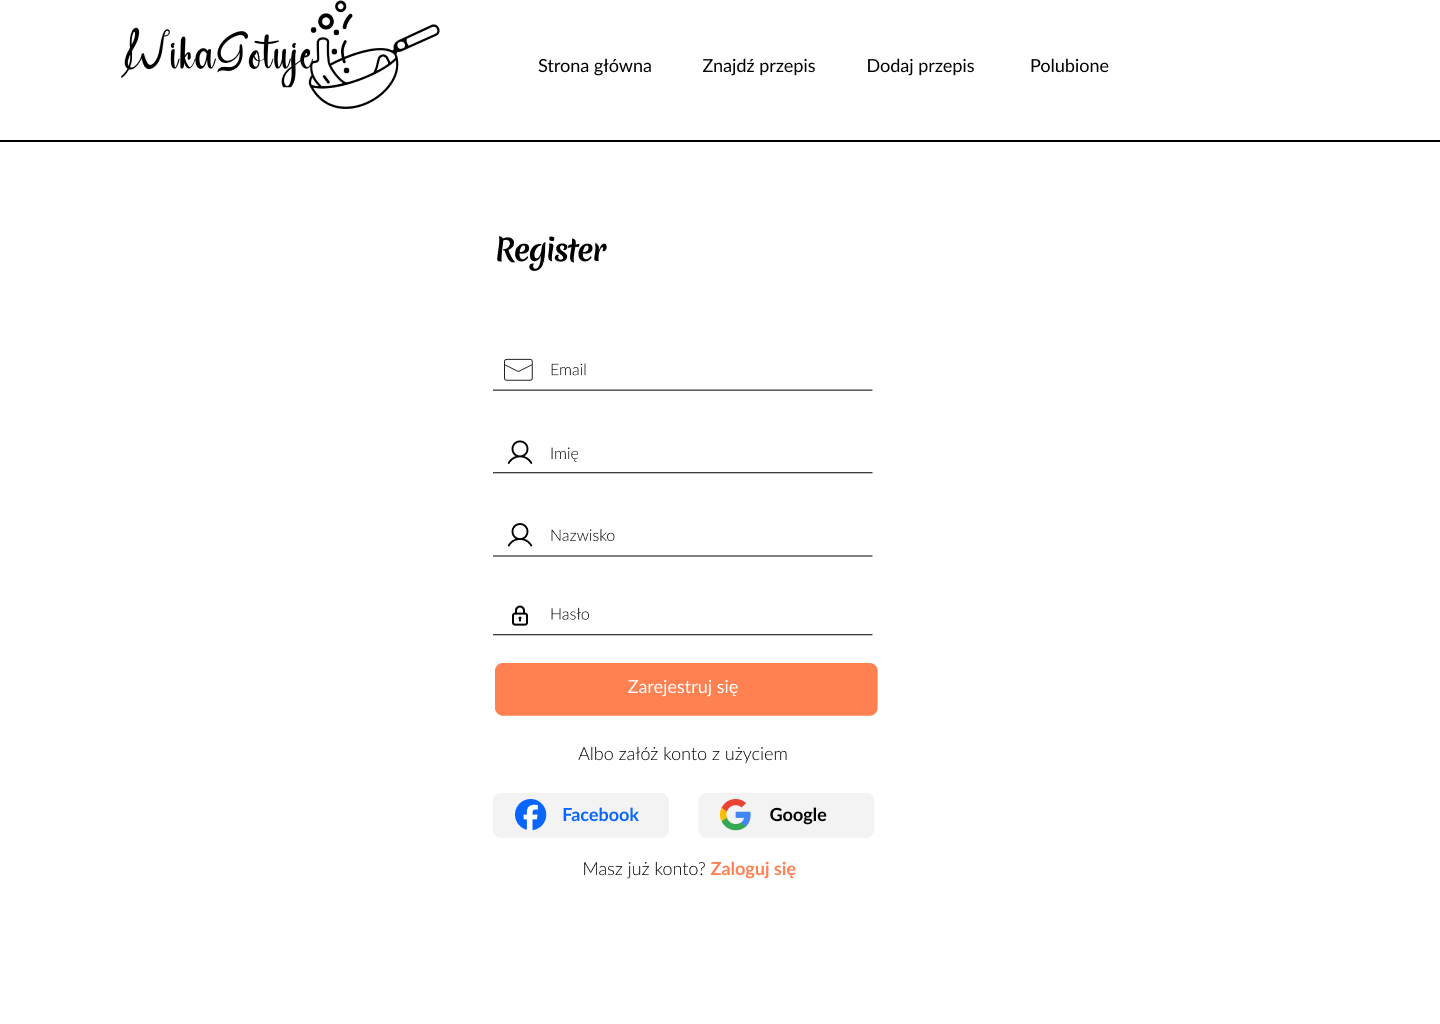
\includegraphics[width=0.8\textwidth]{mockups/register_page}
    \end{center}
    \caption{Widok podstrony odpowiedzialnej za rejestrację nowych użytkowników}
\end{figure}

\section{Scenariusze i storyboardy}
\subsection{Scenariusz 1 - znelezienie przepisu zgodnego z własnymi preferencjami}

Młoda osoba włącza komputer, żeby znaleźć nowy przepis kulinarny. Interesują ją główne dania wegetariańskie pochodzenia azjatyckiego. Nasza osoba ma wolne 2 godziny na przygotowanie 
posiłku i chce ugotować coś ławego, jednocześnie nie odwiedzając dużo sklepów, aby znaleźć potrzebne składniki. Interesują ją najpopularniejsze propozycje.

\subsection{Storyboard}
\begin{enumerate}
    \item Zakładamy, że osoba z naszego scenariusza zaczyna swoje poszukiwania na ekranie głównym naszej witryny internetowej (patrz Rysunek: \ref{fig:main_page})
    \item W kolejnym kroku aktor z naszego scenariusza klika w opcję znajdź przepis z nagłówka 
        \begin{figure}[H]
            \begin{center}
                
\includegraphics[width=0.8\textwidth]{images/find_recipe_step1}
            \end{center}
        \end{figure}
    \item Użytkownikowi ukazuje się ekran filtrowania przepisów (patrz Rysunek: \ref{fig:find_recipe})
    \item Użytkownik wybiera interesujący go typ dania po przez kliknięcie w pole opisane napisem \textit{Rodzaj potrawy} opcji \textit{Danie główne}
        \begin{figure}[H]
            \begin{center}
                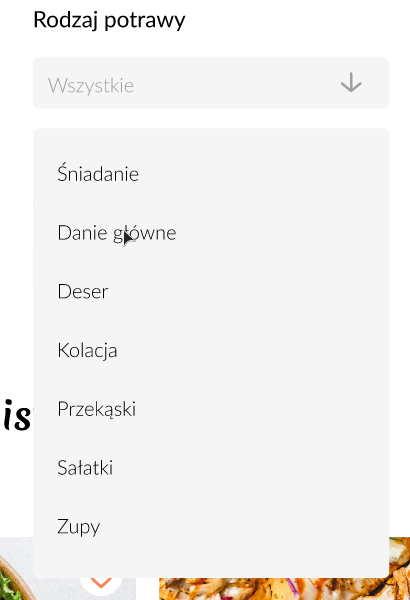
\includegraphics[width=0.3\textwidth]{images/find_recipe_step2}
            \end{center}
        \end{figure}
    \item Następnie użytkownik wybiera, że interesują go łatwe przepisy po przez wybranie odpowiedniej opcji w polu \textit{Poziom zaawansowania}
        \begin{figure}[H]
            \begin{center}
                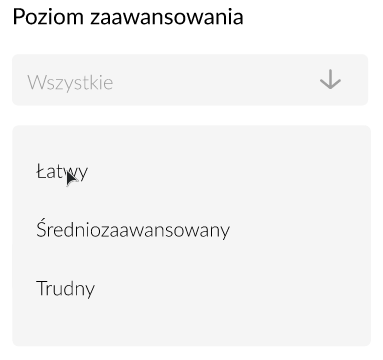
\includegraphics[width=0.3\textwidth]{images/find_recipe_step3}
            \end{center}
        \end{figure}

    \item Aktor z naszego scenariusza nie chce przeszukiwać dużej ilości sklepów więc wybiera \textit{Łatwą dostępność składników} w polu oznakowanym jako \textit{Dostępność składników}
        \begin{figure}[H]
            \begin{center}
                
\includegraphics[width=0.3\textwidth]{images/find_recipe_step4}
            \end{center}
        \end{figure}
    \item Użytkownik jest zainteresowany dietą wegetariańską czyli w polu \textit{Dieta} wybiera \textit{Wegetariańska}
        \begin{figure}[H]
            \begin{center}
                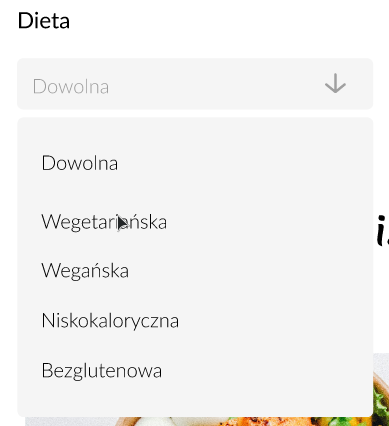
\includegraphics[width=0.3\textwidth]{images/find_recipe_step5}
            \end{center}
        \end{figure}
    \item Użytkownika interesują przepisy, które można zrealizować w maksymalnie 2 godziny. Z tego powodu w polu \textit{Do} oznakowanego opisem \textit{Czas przygotowania} wybiera \textit{120 min}
        \begin{figure}[H]
            \begin{center}
                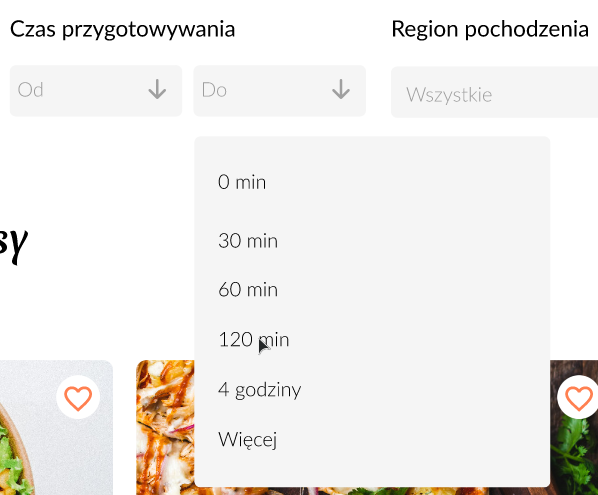
\includegraphics[width=0.4\textwidth]{images/find_recipe_step6}
            \end{center}
        \end{figure}
    \newpage    
    \item Dalej, użytkownik wybiera w polu \textit{Region pochodzenia} pozycję \textit{Azja}
        \begin{figure}[H]
            \begin{center}
                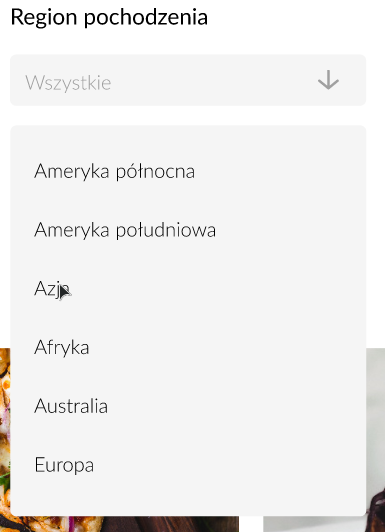
\includegraphics[width=0.3\textwidth]{images/find_recipe_step7}
            \end{center}
        \end{figure}
    \item Na tym etapie nasz użytkownik powinień widzieć już przepisy zgodne z jego preferencjami poniżej filtrów, pamiętajmy jednak, że interesują go najpopularniejsze propozycje.
        Z tego powodu nasz aktor w polu \textit{Sortuj} wybiera opcję \textit{Popularność}.
        \begin{figure}[H]
            \begin{center}
                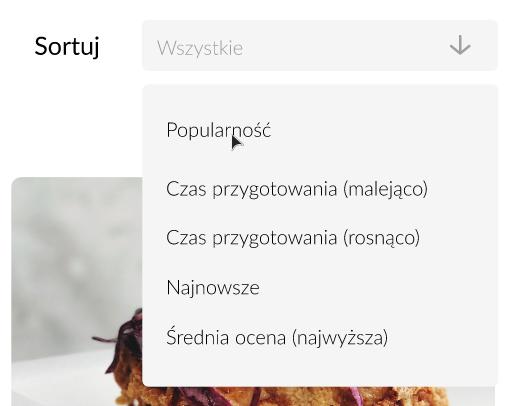
\includegraphics[width=0.3\textwidth]{images/find_recipe_step8}
            \end{center}
        \end{figure}
    \item Po wykonaniu tych kroków użytkownik może zacząć przeglądać zwrócone przez stronę przepisy
\end{enumerate}

\newpage

\subsection{Scenariusz 2 - Dodanie nowego przepisu}
Osoba pochodzenia gruzińskiego chce zachęcić swoich znajomych do przygotowania dania o nazwie \textit{Chinkali} z tradycyjnego gruzińskiego dania. Niestety dostępne w sieci przepisy
w języku polskim nie są poprawne, a jedyna receptura spełniająca kryteria naszej osoby jest w języku gruzińskim. Z tego powodu decyduje się dodać ten przepis w przetłumaczonej
na język polski wersji, a następnie podesłać go znajomym (chce po prostu podesłać do niego link). Osoba z naszego scenariusza przygotowała już kiedyś to danie i posiada jego zdjęcie.
Wie też, że jest to danie główne, przepis pozwala na przygotowanie 4 porcji, zawiera w sobie mięso, a przygotowanie zajmuje mniej więcej 2 godziny. Aktor naszego scenariusza spotkał
już kiedyś witrynę \textit{WikaGotuje} i ma tam założone konto, ale nie jest zalogowany.

\subsection{Storyboard}
\begin{enumerate}
    \item Zakładamy, że osoba z naszego scenariusza zaczyna na ekranie głównym naszej witryny internetowej (patrz Rysunek: \ref{fig:main_page})
    \item W kolejnym kroku aktor z naszego scenariusza klika w przycisk \textit{Zaloguj się} w nagłówku
        \begin{figure}[H]
            \begin{center}
                
\includegraphics[width=0.8\textwidth]{images/add_recipe_step1}
            \end{center}
        \end{figure}
    \item Użytkownikowi ukazuje się ekran logowania (patrz Rysunek: \ref{fig:login_page})
    \item Użytkownik wprowadza dane do swojego konta i klika przycisk \textit{Zaloguj się}
    \item Po zalogowaniu użytkownik wybiera opcję \textit{Dodaj przepis} w nagłówku strony
        \begin{figure}[H]
            \begin{center}
                
\includegraphics[width=0.8\textwidth]{images/add_recipe_step2}
            \end{center}
        \end{figure}
    \item Użytkownikowi ukazuje się strona dodawania przepisu (patrz Rysunek: \ref{fig:add_recipe})
    \item Użytkownik wpisuje \textit{Chinkali} w pole \textit{Nazwa przepisu}
        \begin{figure}[H]
            \begin{center}
                
\includegraphics[width=0.3\textwidth]{images/add_recipe_step3}
            \end{center}
        \end{figure}
    \item Użytkownik wybiera w polu \textit{Rodzaj potrawy} opcję \textit{Danie główne}
        \begin{figure}[H]
            \begin{center}
                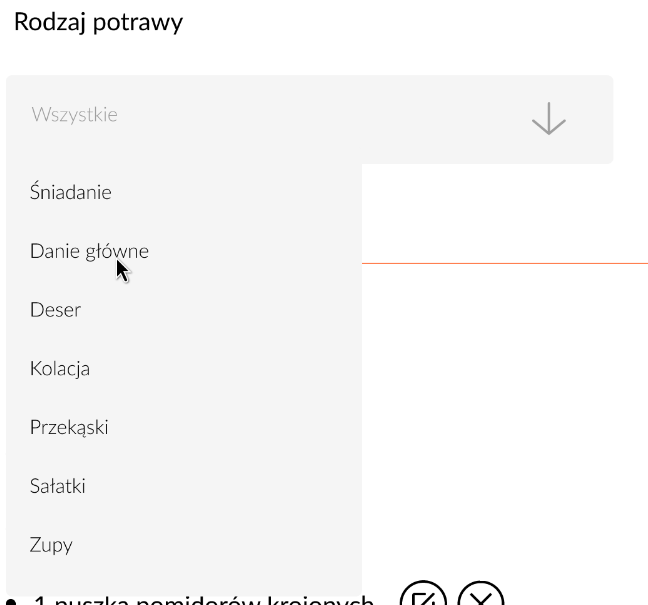
\includegraphics[width=0.3\textwidth]{images/add_recipe_step4}
            \end{center}
        \end{figure}
    \newpage

    \item Użytkownik klika w ikonę zdjęcia w polu \textit{Wybierz zdjęcie}
        \begin{figure}[H]
            \begin{center}
                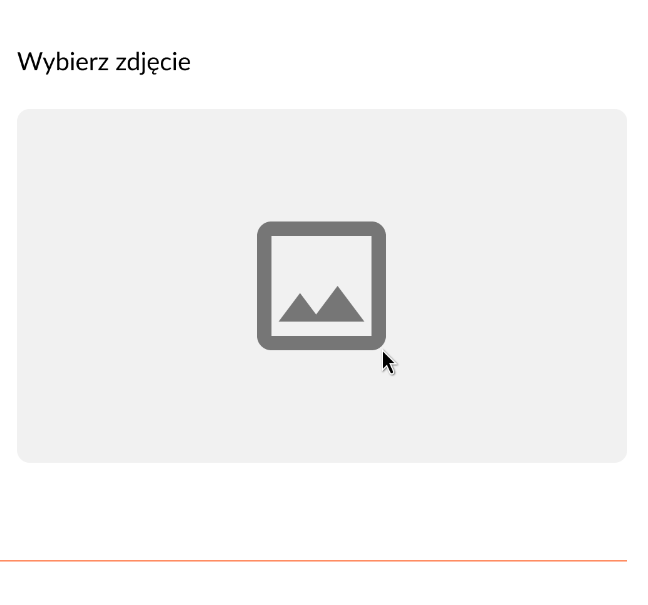
\includegraphics[width=0.3\textwidth]{images/add_recipe_step5}
            \end{center}
        \end{figure}
    \item Użytkownikowi ukazuje się systemowy file picker
    \item Użytkownik wybiera zdjęcie gotowego dania
    \item W sekcji \textit {Potrzebne składniki} dla składniku użytkownik wprowadza jego ilość i nazwę w odpowiednie pole tekstowe i klika symbol +
        \begin{figure}[H]
            \begin{center}
                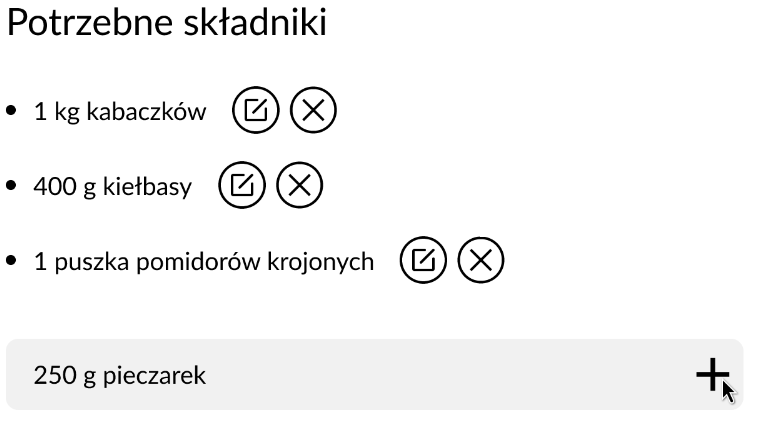
\includegraphics[width=0.3\textwidth]{images/add_recipe_step6}
            \end{center}
        \end{figure}
    \item W sekcji \textit{Lista kroków} dla każdego kroku użytkownik wprowadza jego opis w odpowiednie pole tekstowe i klika symbol +
        \begin{figure}[H]
            \begin{center}
                
\includegraphics[width=0.3\textwidth]{images/add_recipe_step7}
            \end{center}
        \end{figure}
    \item Użytkownik w polu \textit{Poziom zaawansowania} wybiera opcję \textit{Średniozaawansowany}
        \begin{figure}[H]
            \begin{center}
                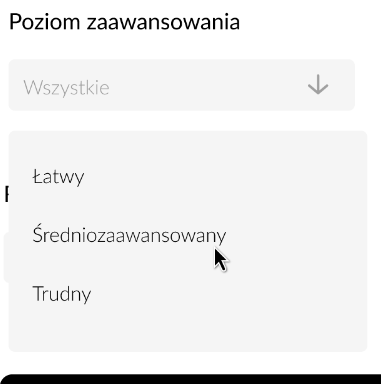
\includegraphics[width=0.3\textwidth]{images/add_recipe_step8}
            \end{center}
        \end{figure}
    \newpage

    \item Użytkownik w polu \textit{Dostępność składników} wybiera opcję \textit{Łatwa dostępność składników}
        \begin{figure}[H]
            \begin{center}
                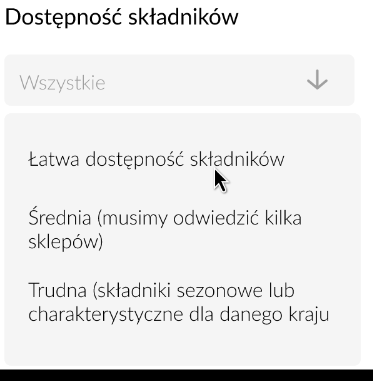
\includegraphics[width=0.3\textwidth]{images/add_recipe_step9}
            \end{center}
        \end{figure}
    \item Użytkownik w polu \textit{Czas przygotowania} wpisuje \textit{120}
        \begin{figure}[H]
            \begin{center}
                
\includegraphics[width=0.3\textwidth]{images/add_recipe_step10}
            \end{center}
        \end{figure}
    \item Użytkownik w polu \textit{Region pochodzenia} wybiera opcję \textit{Europa}
        \begin{figure}[H]
            \begin{center}
                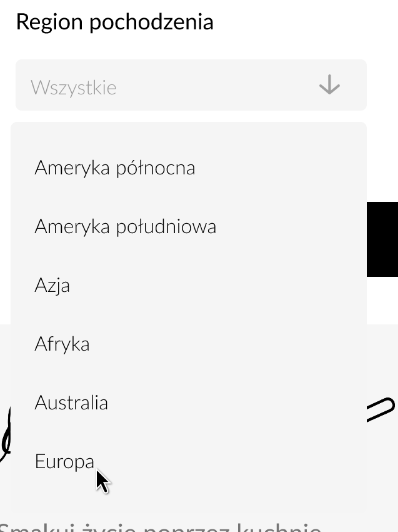
\includegraphics[width=0.3\textwidth]{images/add_recipe_step11}
            \end{center}
        \end{figure}
    \item Użytkownik klika przycisk dodaj przepis na dole strony
        \begin{figure}[H]
            \begin{center}
                
\includegraphics[width=0.8\textwidth]{images/add_recipe_step12}
            \end{center}
        \end{figure}
    \newpage

    \item Po wykonaniu tych kroków użytkownik zostaje przekierowany na stronę z dodanym przepisem. Może teraz skopiować link i wysłać go swoim znajomym
        \begin{figure}[H]
            \begin{center}
                
\includegraphics[width=0.4\textwidth]{images/add_recipe_step13}
            \end{center}
        \end{figure}
\end{enumerate}

\end{document}
